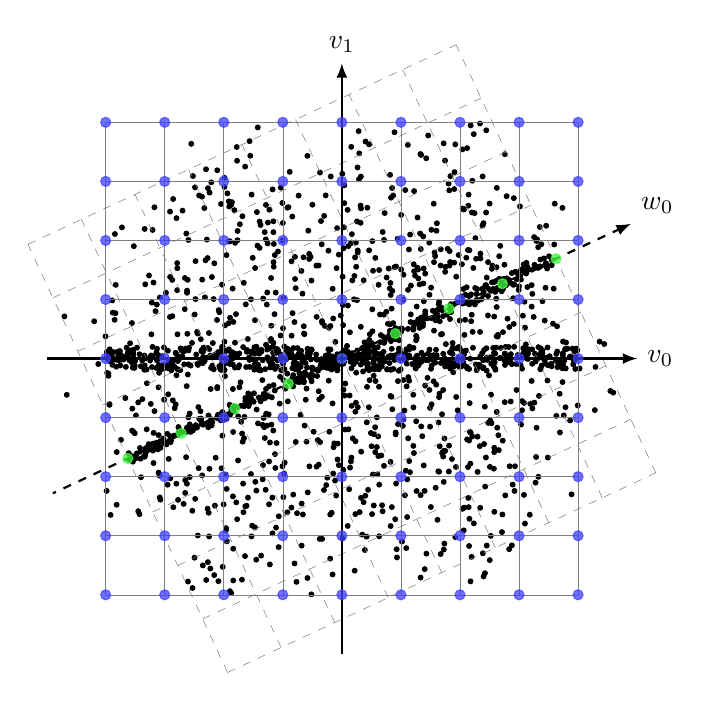
\begin{tikzpicture}[rotate=0,scale=0.75]
	% grid lines
	\def\xmin{-4}
	\def\ymin{-4}
	\def\xmax{4}
	\def\ymax{4}
	\def\xinc{1}
	\def\yinc{1}
	\pgfmathsetmacro{\xcentre}{(\xmax + \xmin) / 2}
	\pgfmathsetmacro{\ycentre}{(\ymax + \ymin) / 2}
	\pgfmathsetmacro{\xnext}{\xmin+\xinc}
	\pgfmathsetmacro{\ynext}{\ymin+\yinc}
	\def\angle{25}

	\def\xvar{3}
	\pgfmathsetmacro{\xvar}{(\xmax - \xmin)/2}
	\pgfmathsetmacro{\xoff}{0}
	\pgfmathsetmacro{\yvar}{\ymax/1.5}
	\pgfmathsetmacro{\yoff}{0}

	% draw random black dots all around
	\foreach \i in {1,2,...,250} {
		% ifthenelse can only compare integers
		\pgfmathsetmacro{\x}{(rand) * \xvar + \xoff}
		\pgfmathsetmacro{\y}{(rand) * \yvar + \yoff}
		\pgfmathtruncatemacro{\dist}{100*abs(\y-sin(\angle)/cos(\angle)*\x}
		\ifthenelse{\dist < 15}{\def\colour{black!40}}{\def\colour{black}}
		\filldraw [black] (\x,\y) circle (0.040);
	}

	\foreach \i in {1,2,...,250} {
		% ifthenelse can only compare integers
		\pgfmathsetmacro{\x}{(rand) * \xvar + \xoff}
		\pgfmathsetmacro{\y}{(rand) * \yvar + \yoff}
		\pgfmathsetmacro{\xrot}{\x*cos(\angle) - \y*sin(\angle)}
		\pgfmathsetmacro{\yrot}{\x*sin(\angle) + \y*cos(\angle)}
		\pgfmathtruncatemacro{\dist}{100*abs(\yrot-sin(\angle)/cos(\angle)*\xrot}
		\ifthenelse{\dist < 25}{\def\colour{black!40}}{\def\colour{black}}
		\filldraw [black] (\xrot,\yrot) circle (0.040);
	}

	\foreach \i in {1,2,...,250} {
		% ifthenelse can only compare integers
		\pgfmathsetmacro{\x}{(rand) * \xvar + \xoff}
		\pgfmathsetmacro{\y}{(rand) * \yvar + \yoff}
		\pgfmathsetmacro{\xrot}{\x*cos(-\angle) - \y*sin(-\angle)}
		\pgfmathsetmacro{\yrot}{\x*sin(-\angle) + \y*cos(-\angle)}
		\pgfmathtruncatemacro{\dist}{100*abs(\yrot-sin(\angle)/cos(\angle)*\xrot}
		\ifthenelse{\dist < 25}{\def\colour{black!40}}{\def\colour{black}}
		\filldraw [black] (\xrot,\yrot) circle (0.040);
	}

	\foreach \i in {1,2,...,250} {
		% ifthenelse can only compare integers
		\pgfmathsetmacro{\x}{(rand) * \xvar + \xoff}
		\pgfmathsetmacro{\y}{(rand) * \yvar + \yoff}
		\pgfmathsetmacro{\xrot}{\x*cos(90) - \y*sin(90)}
		\pgfmathsetmacro{\yrot}{\x*sin(90) + \y*cos(90)}
		\pgfmathtruncatemacro{\dist}{100*abs(\yrot-sin(\angle)/cos(\angle)*\xrot}
		\ifthenelse{\dist < 25}{\def\colour{black!40}}{\def\colour{black}}
		\filldraw [black] (\xrot,\yrot) circle (0.040);
	}

	% draw gray dots around main axis
	\pgfmathsetmacro{\yvar}{0.20}
	\foreach \i in {1,2,...,500} {
		% ifthenelse can only compare integers
		\pgfmathsetmacro{\x}{(rand) * \xvar + \xoff}
		\pgfmathsetmacro{\y}{(rand) * \yvar + \yoff}
		%\shade [ball color = black, opacity = 1] (\x,\y) circle (0.040);
		\filldraw [black] (\x,\y) circle (0.040);
	}

	% draw random red dots around secondary helper axis
	\draw[style=help lines, dashed, very thin, rotate=\angle] (\xmin,\ymin) grid (\xmax,\ymax);
	\draw[-latex,thick,dashed] (\xcentre,\ycentre) --++ (\angle:\xmax+1.4) node [above right]{$w_0$};
	\draw[thick,dashed,] (\xcentre,\ycentre) --++ (\angle:-\xmax-1.4);
	\pgfmathsetmacro{\yvar}{0.10}
	\foreach \i in {1,2,...,300} {
		\pgfmathsetmacro{\x}{(rand) * \xvar + \xoff}
		\pgfmathsetmacro{\y}{(rand) * \yvar + \yoff}
		\pgfmathsetmacro{\xrot}{\x*cos(\angle) - \y*sin(\angle)}
		\pgfmathsetmacro{\yrot}{\x*sin(\angle) + \y*cos(\angle)}
		\pgfmathsetmacro{\radius}{3}
		\pgfmathtruncatemacro{\smallcircle}{10 * (\x*\x + \y*\y) - \radius}
		\ifthenelse{\smallcircle < 0}{\def\colour{black}}{\def\colour{black!40}}
		\filldraw [black] (\xrot,\yrot) circle (0.040);
	}

	% draw axis for secondary helper transform
	\foreach \x in {\xmin,\xnext,...,\xmax} {
			\pgfmathsetmacro{\xrot}{\x*cos(\angle)}
			\pgfmathsetmacro{\yrot}{\x*sin(\angle)}
			\filldraw [green!75, opacity = 0.75] (\xrot,\yrot) circle (0.085);
	}

	\draw[style=help lines, very thin] (\xmin,\ymin) grid (\xmax,\ymax);
	% main axis
	\draw[-latex, thick] (\xmin-1,\ycentre) -- (\xmax+1,\ycentre) node[right] {$v_0$};
	\draw[-latex, thick] (\xcentre,\ymin-1) -- (\xcentre,\ymax+1) node[above] {$v_1$};
	\pgfmathsetseed{5}
	
	\foreach \x in {\xmin,\xnext,...,\xmax} {
		\foreach \y in {\ymin,\ynext,...,\ymax} {
			\filldraw [blue!75, opacity = 0.75] (\x,\y) circle (0.085);
		}
	}

\end{tikzpicture}
